%%%%%%%%%%%%%%%%%%%%%%%%%%%%%%%%%%%%%%%%%%%%%%%%%%%%%%%%%%%%%%%%%%%%%%%%%%%%%%%%
%% LaTeX sources for The Guide to Software Engineering & Professional Practice
%% Michael B. Gale (m.gale@bham.ac.uk)
%%
%% This work is licensed under the Creative Commons
%% Attribution-NonCommercial-NoDerivatives 4.0 International License. To
%% view a copy of this license, visit
%% http://creativecommons.org/licenses/by-nc-nd/4.0/ or send a letter to
%% Creative Commons, PO Box 1866, Mountain View, CA 94042, USA.
%%%%%%%%%%%%%%%%%%%%%%%%%%%%%%%%%%%%%%%%%%%%%%%%%%%%%%%%%%%%%%%%%%%%%%%%%%%%%%%%

\documentclass[12pt,a4paper,twoside,fleqn]{report}

\usepackage{geometry}
\usepackage[latin1]{inputenc}
\usepackage{amsmath}
\usepackage{amsfonts}
\usepackage{amssymb}
\usepackage{graphicx}
\usepackage{fancyeq}
\usepackage{fancyhdr}
\usepackage[explicit]{titlesec}
\usepackage{color}
\usepackage{longtable}
\usepackage{array, booktabs}
\usepackage{colortbl}
\usepackage{wrapfig}
\usepackage{pgfplots}
\usepackage[strict]{changepage}
\usepackage{graphbox}
\usepackage{prerex}
\usepackage{forest}
\usepackage{multicol}
\usepackage{fontawesome}
\usepackage{natbib}
\usepackage{ccicons}

% Minted -------------------------------

\usepackage{minted}
\usepackage[
backgroundcolor = gray!5
, hidealllines=true
]{mdframed}

\surroundwithmdframed{minted}
\usemintedstyle{lovelace}

\setminted[text]{fontsize=\small}
\setminted[haskell]{fontsize=\small}
\setminted[bash]{fontsize=\small}
\newcommand{\haskellIn}[1]{\mintinline[fontsize=\small]{haskell}{#1}}
\newcommand{\bashIn}[1]{\mintinline[fontsize=\small]{bash}{#1}}

% Tikz -------------------------------

\usepackage{tikz}
\usetikzlibrary{arrows}

\tikzset{
	treenode/.style = {align=center, inner sep=0pt, text centered,
		font=\sffamily},
	arn_n/.style = {treenode, circle, white, font=\sffamily\bfseries, draw=black,
		fill=black, text width=1.5em},
	arn_r/.style = {treenode, circle, red, draw=red,
		text width=1.5em, very thick},
	arn_x/.style = {treenode, circle, draw=white,
		minimum width=1.5em, minimum height=1.5em},
	cls/.style = { treenode, rectangle, red, draw=red,
		text width=1.5em, very thick, minimum width=1.5em, minimum height=1.5em }
}

% UK English -------------------------------
\usepackage[UKenglish]{babel}
\usepackage[UKenglish]{isodate}

% Hyperref -------------------------------
\usepackage{hyperref}
\hypersetup{
    colorlinks=true,
    linkcolor=black,
    urlcolor=black,
    citecolor=black,
    unicode=false
}

% cleveref
\usepackage[nameinlink]{cleveref}

\crefname{figure}{figure}{figures} % cleveref by default has `fig.'
\Crefname{figure}{Figure}{Figures}

\crefname{section}{section}{sections} % cleveref by default has `fig.'
\Crefname{section}{Section}{Sections}

% Fonts -------------------------------
\usepackage[]{FiraSans}

% Palatino (font)
\usepackage{mathpazo}
\linespread{1.05}         % Palatino needs more leading (space between lines)
\usepackage[T1]{fontenc}

% some format settings
% for hard-bound final submission, use:
%\setlength{\oddsidemargin}{4.6mm}     % 30 mm left margin - 1 in
% for soft-bound version and techreport, use instead:
\setlength{\oddsidemargin}{-0.4mm}    % 25 mm left margin - 1 in
\setlength{\evensidemargin}{-0.4mm}
\setlength{\topmargin}{-5.4mm}        % 20 mm top margin - 1 in
\setlength{\textwidth}{160mm}         % 20/25 mm right margin
\setlength{\textheight}{237mm}        % 20 mm bottom margin
\setlength{\headheight}{5mm}
\setlength{\headsep}{5mm}
\setlength{\parindent}{0mm}
\setlength{\parskip}{\medskipamount}
\renewcommand\baselinestretch{1.2} % thesis format (not needed for techreport)
% don't let large figures hijack entire pages
\renewcommand\topfraction{.9}
\renewcommand\textfraction{.1}
\renewcommand\floatpagefraction{.8}

\usepackage[nomap]{FiraMono}

\usepackage{microtype}
\DisableLigatures[f]{encoding = *, family = tt* }

\author{Michael B. Gale}


\definecolor{gray75}{gray}{0.75}
\newcommand{\hsp}{\hspace{20pt}}

\titleformat{name=\chapter}[hang]{}{}{0cm}{%
	\protect\thispagestyle{fancy}
	\begin{center}
		\large $\lambda$.\thechapter \\
		\huge \textsc{#1}
	\end{center}
	%\chaptermark{\chapter}
}
\titleformat{name=\chapter,numberless}[hang]{}{}{0cm}{%
	\begin{center}
		\huge \textsc{#1}
	\end{center}
	%\chaptermark{\chapter}
}

%\titleformat{\subsection}{format}{label}{0em}{before-code}

\titleformat{\section}
	{\bfseries\large}
	{\llap{\parbox{1.5cm}{\thesection\hfill}}#1}
	{0em}
	{\bfseries}

\titleformat{\subsection}
{\bfseries}{\llap{\parbox{1.5cm}{\thesubsection\hfill}}#1}{0em}{\bfseries}


% misc. commands
\newcounter{TaskCounter}

\newcommand{\question}[1]{\vspace{-0.7cm}{\footnotesize \emph{#1}} \vspace{0.25cm}}
\newcommand{\topics}[1]{\vspace{-0.5cm}{\footnotesize \emph{Topics}: #1} \vspace{0.25cm}}
\newcommand{\task}[2][]{\indent\llap{\parbox{1.5cm}{\refstepcounter{TaskCounter}\label{#1}{\firamedium Ex\theTaskCounter}\hfill}}#2}
\newcommand{\solution}[2]{\indent\llap{\parbox{1.5cm}{\textbf{Ex#1}\hfill}}#2}
\newcommand{\taskLine}{\bigskip\hrule\bigskip}

\AtBeginDocument{\addtocontents{toc}{\protect\thispagestyle{fancy}}}

%%%%%%%%%%%%%%%%%%%%%%%%%%%%%%%%%%%%%%%%%%%%%%%%%%%%%%%%%%%%%%%%%%%%%%%%%%%%%%%%
%% LaTeX sources for The Guide to Software Engineering & Professional Practice
%% Michael B. Gale (m.gale@bham.ac.uk)
%%
%% This work is licensed under the Creative Commons
%% Attribution-NonCommercial-NoDerivatives 4.0 International License. To
%% view a copy of this license, visit
%% http://creativecommons.org/licenses/by-nc-nd/4.0/ or send a letter to
%% Creative Commons, PO Box 1866, Mountain View, CA 94042, USA.
%%%%%%%%%%%%%%%%%%%%%%%%%%%%%%%%%%%%%%%%%%%%%%%%%%%%%%%%%%%%%%%%%%%%%%%%%%%%%%%%

% Names for organisations, products, etc.
\newcommand{\ssh}{SSH}
\newcommand{\sshShortName}{Student Smart Homes}
\newcommand{\sshFullName}{\sshShortName\ (\ssh)}
\newcommand{\sshHubShort}{\ssh\ Hub}
\newcommand{\sshHub}{\sshHubShort\ - First Class}
\newcommand{\sshCloud}{\ssh\ Cloud}
\newcommand{\sshCamera}{\ssh\ Camera}
\newcommand{\sshApp}{\ssh\ App}
\newcommand{\sshConsole}{\ssh\ Console Table}

\newcommand{\higherEdFullName}{Higher Education Software Solutions Plc}
\newcommand{\higherEdShortName}{Higher Education Software Solutions}
\newcommand{\higherEdCSRS}{CSRS}
\newcommand{\higherEdAntiCheat}{RewriteItIn}


\begin{document}
\fancypagestyle{empty}{\fancyhf{}}
\pagestyle{empty}
\pagenumbering{roman}

\renewcommand{\headrulewidth}{0pt}
\renewcommand{\footrulewidth}{0pt}

%%%%%%%%%%%%%%%%%%%%%%%%%%%%%%%%%%%%%%%%%%%%%%%%%%%%%%%%%%%%%%%%%%%%%%%%%%%%%%%%
%% LaTeX sources for The Guide to Software Engineering & Professional Practice
%% Michael B. Gale (m.gale@bham.ac.uk)
%%
%% This work is licensed under the Creative Commons
%% Attribution-NonCommercial-NoDerivatives 4.0 International License. To
%% view a copy of this license, visit
%% http://creativecommons.org/licenses/by-nc-nd/4.0/ or send a letter to
%% Creative Commons, PO Box 1866, Mountain View, CA 94042, USA.
%%%%%%%%%%%%%%%%%%%%%%%%%%%%%%%%%%%%%%%%%%%%%%%%%%%%%%%%%%%%%%%%%%%%%%%%%%%%%%%%

\begin{titlepage}
	\begin{center}

{\Huge \textit{The guide to}} \\[0.2cm]
{\Huge \textbf{Software Engineering \&\\ Professional Practice}} \\[0.2cm]

\vfill

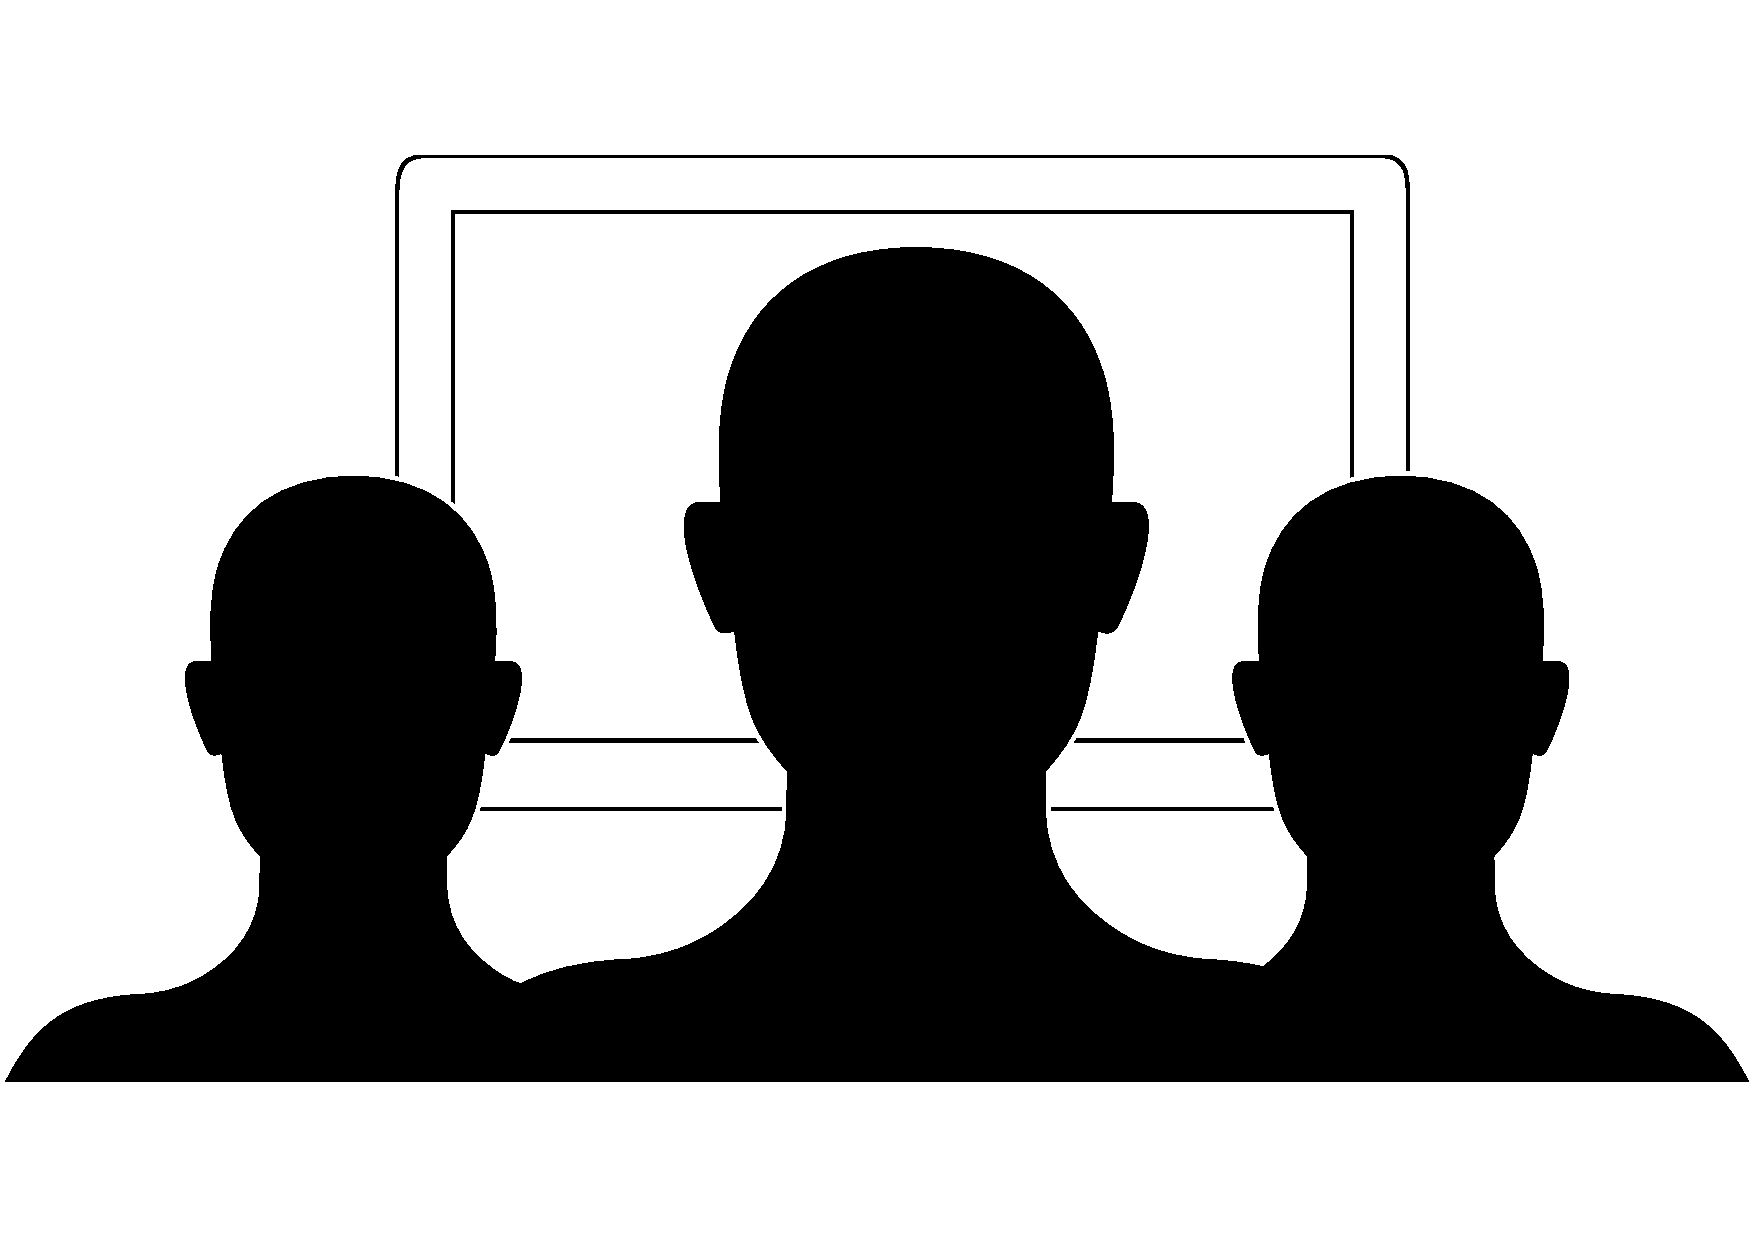
\includegraphics[scale=0.53]{logo-bw.pdf}

\vfill

{\LARGE Michael B. Gale} \\[0.1cm]
{\large \href{mailto:m.gale@bham.ac.uk}{m.gale@bham.ac.uk}}

\vspace{1cm}

{\Large 2024/25}
\end{center}
\end{titlepage}

\phantom{~}
\vfill

\ccbyncnd

\vspace*{0.2cm}

This work is licensed under a Creative Commons\\
Attribution-NonCommercial-NoDerivatives 4.0 International License.

\vspace*{0.2cm}

\url{http://creativecommons.org/licenses/by-nc-nd/4.0/}


\cleardoublepage
%\setcounter{page}{1}

\fancyhf{}
\fancyhead[LE, RO]{\emph{The Guide to Software Engineering \& Professional Practice}}
\fancyhead[LO, RE]{\emph{Michael B. Gale}}

\fancyfoot[LE,RO]{\thepage}
\pagestyle{fancy}
\thispagestyle{fancy}
\newgeometry{
	tmargin=2.5cm,
	textwidth=155mm,
	textheight=247mm,
	headheight=5mm,
	headsep=5mm,
	inner=30mm
}

\tableofcontents


\cleardoublepage
\pagenumbering{arabic}

%%%%%%%%%%%%%%%%%%%%%%%%%%%%%%%%%%%%%%%%%%%%%%%%%%%%%%%%%%%%%%%%%%%%%%%%%%%%%%%%
%% LaTeX sources for The Guide to Software Engineering & Professional Practice
%% Michael B. Gale (m.gale@bham.ac.uk)
%%
%% This work is licensed under the Creative Commons
%% Attribution-NonCommercial-NoDerivatives 4.0 International License. To
%% view a copy of this license, visit
%% http://creativecommons.org/licenses/by-nc-nd/4.0/ or send a letter to
%% Creative Commons, PO Box 1866, Mountain View, CA 94042, USA.
%%%%%%%%%%%%%%%%%%%%%%%%%%%%%%%%%%%%%%%%%%%%%%%%%%%%%%%%%%%%%%%%%%%%%%%%%%%%%%%%

\chapter{The Module}

For many of you, a degree in Computer Science will be the stepping stone to a career in software engineering. At the same time, most of your experience building software has been to write some Java code on your own, compile it directly with the Java compiler, and run it on your own machine. Real software engineering is very different.

In this module, we will explore the gap between the programming you will have done in your first year and the real software engineering you are likely to do in your careers. You will be introduced to the different contexts that software engineering takes place in and the different processes that organisations may employ surrounding it. Furthermore, you will gain foundational knowledge of relevant tools and technical skills.

This guide serves as a companion to the module by giving you an overview of all the major components. It will be a living document that will evolve to include more content as the module progresses.

%%%%%%%%%%%%%%%%%%%%%%%%%%%%%%%%%%%%%%%%%%%%%%%%%%%%%%%%%%%%%%%%%%%%%%%%%%%%%%%%
%% LaTeX sources for The Guide to Software Engineering & Professional Practice
%% Michael B. Gale (m.gale@bham.ac.uk)
%%
%% This work is licensed under the Creative Commons
%% Attribution-NonCommercial-NoDerivatives 4.0 International License. To
%% view a copy of this license, visit
%% http://creativecommons.org/licenses/by-nc-nd/4.0/ or send a letter to
%% Creative Commons, PO Box 1866, Mountain View, CA 94042, USA.
%%%%%%%%%%%%%%%%%%%%%%%%%%%%%%%%%%%%%%%%%%%%%%%%%%%%%%%%%%%%%%%%%%%%%%%%%%%%%%%%

\section{Recommended reading}

You are not required to purchase any books for this module as there are many free resources available online. As we focus on covering a breadth of topics, rather than a single topic in great depth, I will make individual recommendations for each week.

%%%%%%%%%%%%%%%%%%%%%%%%%%%%%%%%%%%%%%%%%%%%%%%%%%%%%%%%%%%%%%%%%%%%%%%%%%%%%%%%
%% LaTeX sources for The Guide to Software Engineering & Professional Practice
%% Michael B. Gale (m.gale@bham.ac.uk)
%%
%% This work is licensed under the Creative Commons
%% Attribution-NonCommercial-NoDerivatives 4.0 International License. To
%% view a copy of this license, visit
%% http://creativecommons.org/licenses/by-nc-nd/4.0/ or send a letter to
%% Creative Commons, PO Box 1866, Mountain View, CA 94042, USA.
%%%%%%%%%%%%%%%%%%%%%%%%%%%%%%%%%%%%%%%%%%%%%%%%%%%%%%%%%%%%%%%%%%%%%%%%%%%%%%%%

\section{Timeline}
\label{sec:timeline}

This module is comprised of approximately 22 lectures and 3 pieces of coursework. This section contains a chronological schedule of all of these components. Note that the schedule may be subject to changes due to \emph{e.g.} staff illness or other unforeseen circumstances. Each lecture aims to answer a specific question, which is shown in the timeline. You can test your understanding by asking yourself that question after each lecture and checking that you can answer it.

\newcommand{\foo}{\makebox[0pt]{\textbullet}\hskip-0.5pt\vrule width 1pt\hspace{\labelsep}}

\newcommand{\LectureEntry}[4]{#1 & \begin{tabular}{p{11cm}}
		\textbf{#2} \\[-0.15cm]
		\emph{#3} \\
		#4
\end{tabular}}
\newcommand{\LabEntry}[3]{#1 & \begin{tabular}{p{11cm}}
		\textbf{#2} \\
		#3
\end{tabular}}

\begingroup
%\begin{table}
\newcommand{\oldarraystrech}{\arraystretch}
	\renewcommand\arraystretch{1.4}\vskip-1.5ex
	\begin{longtable}{@{\,}r <{\hskip 2pt} !{\foo} >{\raggedright\arraybackslash}p{12cm}}
		\addlinespace[1.5ex]
		\LectureEntry{2 October}{Lecture 1: Introduction}{What is this module about?}{Module overview, different settings for software engineering} \\
		\LectureEntry{2 October}{Lecture 2: Classic software engineering techniques}{What are traditional software engineering techniques?}{Waterfall, Spiral, Agile, Prototyping, UML, ...} \\

		\LectureEntry{9 October}{Lecture 3: Technical overview of a software project}{How is a software project organised?}{Introductions to software architectures, code repositories, build tools, dependency management, continuous integration, deployments, ...} \\
        \LectureEntry{9 October}{Lecture 4: How engineering teams work}{How do engineering teams work?}{Engineering design reviews (EDRs), Architecture Design Records (ADRs), units of work, Directly Responsible Individuals, retrospectives, ...} \\

		\LectureEntry{16 October}{Lecture 5: The humans}{What are human aspects that engineers need to be aware of?}{Users, customers, sales teams, field teams, accessibility, internationalisation, ...} \\
		\LectureEntry{16 October}{Lecture 6: Effective technical writing}{How can we communicate technical information effectively?}{Good style, common mistakes, examples of good and bad writing, ...} \\

		\LectureEntry{23 October}{Lecture 7: Observability}{How do you know what's going on with your software?}{Logging, metrics, alerting, ...} \\
		\LectureEntry{23 October}{Lecture 8: Data analytics for Software Engineers}{How can we use data to inform planning decisions and review impact?}{Where and why to leverage data, engineering with data, ...} \\

        \hline
		Week 5 & \begin{tabular}{p{13cm}}
			\textbf{Deadline: Coursework I}
		\end{tabular}\\
		\hline

		\LectureEntry{30 October}{Lecture 9: Stop calling it \texttt{\small \_Version14ReallyFinal.docx}}{How can we use version control effectively?}{Version control systems, Git basics, undoing things, ...} \\
		\LectureEntry{30 October}{Lecture 10: Version control for teams}{How can teams leverage version control to collaborate?}{Common workflows, branches, merging, rebasing, conflicts, ...} \\

		\LectureEntry{6 November}{Lecture 11: Build tools}{How is real software built?}{Build tools, automating builds, managing dependencies, build caching, reproducible builds, ...} \\
		\LectureEntry{6 November}{Lecture 12: Continuous integration}{What is continuous integration and how does it help us?}{Continuous integration systems, examples, deployments, ...} \\

		\LectureEntry{13 November}{Lecture 13: Basic testing}{What are some essential techniques for testing code?}{Testing frameworks, unit tests, integration tests, ...} \\
		\LectureEntry{13 November}{Lecture 14: Not-so-basic testing}{What are some more sophisticated testing techniques?}{Property-based testing, proofs, mocking, designing implementations for testing, ...} \\

		\LectureEntry{20 November}{Lecture 15: Containerisation}{What is containerisation and how is it useful?}{Docker-style containerisation, examples, ...} \\
		\LectureEntry{20 November}{Lecture 16: Orchestration}{Given a bunch of containers and a bunch of servers, how do we run them?}{Kubernetes and friends.} \\

		\LectureEntry{27 November}{Lecture 17: Threat modelling}{How do we incorporate security into the software engineering process?}{What is threat modelling, when to threat-model, different strategies, ...} \\
		\LectureEntry{27 November}{Lecture 18: Supply-chain security}{How do we ensure none of our dependencies have security vulnerabilities?}{Vendoring dependencies, security aduits, vulnerability databases, automatic dependency updates, ...} \\

		\LectureEntry{4 December}{Lecture 19: Static analysis}{How can we check source code for security vulnerabilities?}{What static analysis tools are, how they work, and examples of one in action.} \\
		\LectureEntry{4 December}{Lecture 20: Generative AI as a tool}{Is generative AI going to replace all of us?}{Examples of how generative AI can assist in the software engineering process.} \\

		\hline
		Week 11 & \begin{tabular}{p{13cm}}
			\textbf{Deadlines: Coursework II \& III}
		\end{tabular}\\
		\hline

		\LectureEntry{11 December}{Lecture 21: Open-source}{What considerations are there for using or contributing to open-source projects?}{Licensing, contributing, benefits, ...} \\
		\LectureEntry{11 December}{Lecture 22: Conclusions}{What have we learnt about software engineering?}{Summary of the module and other general information.} \\

	\end{longtable}
%\end{table}
\endgroup

%%%%%%%%%%%%%%%%%%%%%%%%%%%%%%%%%%%%%%%%%%%%%%%%%%%%%%%%%%%%%%%%%%%%%%%%%%%%%%%%
%% LaTeX sources for The Guide to Software Engineering & Professional Practice
%% Michael B. Gale (m.gale@bham.ac.uk)
%%
%% This work is licensed under the Creative Commons
%% Attribution-NonCommercial-NoDerivatives 4.0 International License. To
%% view a copy of this license, visit
%% http://creativecommons.org/licenses/by-nc-nd/4.0/ or send a letter to
%% Creative Commons, PO Box 1866, Mountain View, CA 94042, USA.
%%%%%%%%%%%%%%%%%%%%%%%%%%%%%%%%%%%%%%%%%%%%%%%%%%%%%%%%%%%%%%%%%%%%%%%%%%%%%%%%

\section{Coursework}

There are three pieces of coursework which you will have to complete. You will receive feedback for the first coursework before the second and third coursework are due.

\subsection{The Engineering Design Review (40\%)}

\paragraph{Description} You get to write an \emph{Engineering Design Review} (EDR). An EDR is a document, written by a software engineer, which discusses a proposed design for new functionality in a software system. The document is primarily aimed at other engineers, but also engineering or product managers. An EDR is an opportunity to propose a solution to a problem, discuss your chosen design, explain why you chose it over alternatives, and propose how work on implementing it should be structured.

\paragraph{Aims} This coursework is designed to develop your ability to research a technical problem, propose a solution to it, think about the context in a wider project and organisation, and exercise your technical writing skills.

\subsection{The Prototype (40\%)}

\paragraph{Description} As a small group of 3-4, you will implement a \emph{prototype} based on \emph{one} of your EDRs from the first coursework. A prototype is an as-simple-as-possible implementation of your design that can demonstrate that your design is feasible. In other words, while the goal of your EDR is to describe a solution that makes sense to you and other engineers in theory, the goal of the prototype is to demonstrate that the design holds up once implemented, and no more.

\paragraph{Aims} This tests your ability to collaborate as a small team, choose appropriate implementation tools for your prototype, implement a design, and simulate interfaces and dependencies that your prototype relies on, but which do not actually exist.

\subsection{The Reflections (20\%)}

\paragraph{Description} On your own, you will write a short document reflecting on your participation in the module. By ``reflecting'', we mean ``thinking constructively about''. Reflecting on your development as an individual is a useful skill in any career path. Additionally, organisations may, in one way or another, also ask you to reflect on your development in the context of your employment. This can either be used to help you work towards your career goals, or factor into formal rewards conversations (conversations about salary increases, bonuses, etc.). In addition to reflecting about your own development and work, you may also reflect about colleagues, your team, the organisation you work for, etc.

\paragraph{Aims} Software engineering requires many different skills and, naturally, we are better at some than others. By reflecting on your work, you can figure out which skills you can leverage more strongly to benefit from, and which skills you need to work on going forward. This coursework tests your ability to think constructively about your work, development, and factors that contribute to it.

%%%%%%%%%%%%%%%%%%%%%%%%%%%%%%%%%%%%%%%%%%%%%%%%%%%%%%%%%%%%%%%%%%%%%%%%%%%%%%%%
%% LaTeX sources for The Guide to Software Engineering & Professional Practice
%% Michael B. Gale (m.gale@bham.ac.uk)
%%
%% This work is licensed under the Creative Commons
%% Attribution-NonCommercial-NoDerivatives 4.0 International License. To
%% view a copy of this license, visit
%% http://creativecommons.org/licenses/by-nc-nd/4.0/ or send a letter to
%% Creative Commons, PO Box 1866, Mountain View, CA 94042, USA.
%%%%%%%%%%%%%%%%%%%%%%%%%%%%%%%%%%%%%%%%%%%%%%%%%%%%%%%%%%%%%%%%%%%%%%%%%%%%%%%%

\cleardoublepage
\chapter{Coursework}


\end{document}
